\documentclass[border=15pt]{standalone}
\usepackage{tikz}
\usetikzlibrary{arrows.meta, positioning, calc}

\begin{document}
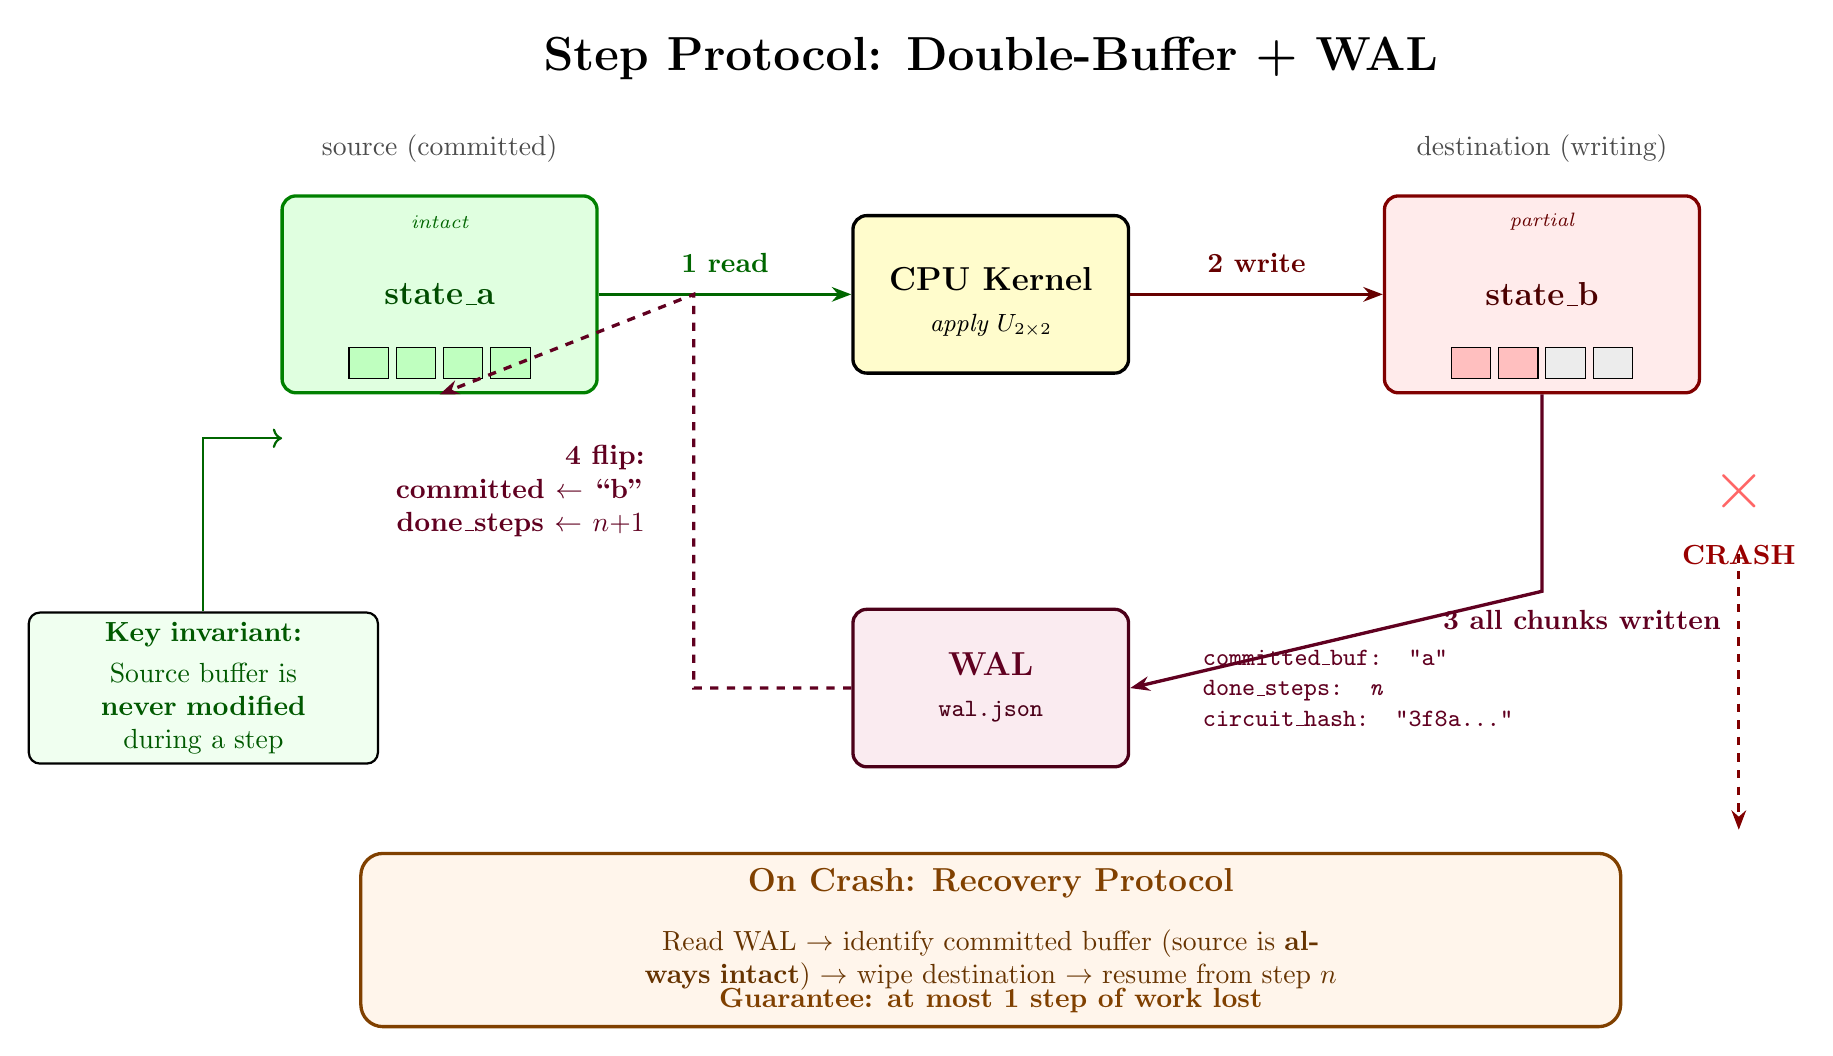
\begin{tikzpicture}[
    myarrow/.style={-{Stealth[length=7pt]}, very thick},
    heading/.style={font=\LARGE\bfseries},
]

% ===================== TITLE =====================
\node[heading] at (7, 12) {Step Protocol: Double-Buffer + WAL};

% ===================== SOURCE BUFFER =====================
\node[draw, very thick, fill=green!12, draw=green!50!black,
      minimum width=4cm, minimum height=2.5cm, rounded corners=5pt]
      (src) at (0, 9) {};
\node[font=\large\bfseries, text=green!30!black] at (src.center) {state\_a};

% Chunk squares inside source
\foreach \i in {0,1,2,3} {
    \node[draw, thin, fill=green!25, minimum width=0.5cm, minimum height=0.4cm]
        at ($(src.south) + (-0.9 + \i*0.6, 0.4)$) {};
}
\node[font=\scriptsize\itshape, text=green!40!black] at ($(src.north) + (0, -0.35)$) {intact};

% Label above
\node[font=\normalsize, text=gray!60!black, above=8pt of src.north] {source (committed)};

% ===================== CPU KERNEL =====================
\node[draw, very thick, fill=yellow!20, rounded corners=5pt,
      minimum width=3.5cm, minimum height=2cm]
      (kern) at (7, 9) {};
\node[font=\large\bfseries] at ($(kern.center) + (0, 0.2)$) {CPU Kernel};
\node[font=\small\itshape] at ($(kern.center) + (0, -0.4)$) {apply $U_{2\times 2}$};

% ===================== DESTINATION BUFFER =====================
\node[draw, very thick, fill=red!8, draw=red!50!black,
      minimum width=4cm, minimum height=2.5cm, rounded corners=5pt]
      (dst) at (14, 9) {};
\node[font=\large\bfseries, text=red!30!black] at (dst.center) {state\_b};

% Chunk squares inside dest (2 written, 2 empty)
\foreach \i/\c in {0/red!25, 1/red!25, 2/gray!15, 3/gray!15} {
    \node[draw, thin, fill=\c, minimum width=0.5cm, minimum height=0.4cm]
        at ($(dst.south) + (-0.9 + \i*0.6, 0.4)$) {};
}
\node[font=\scriptsize\itshape, text=red!40!black] at ($(dst.north) + (0, -0.35)$) {partial};

% Label above
\node[font=\normalsize, text=gray!60!black, above=8pt of dst.north] {destination (writing)};

% ===================== FLOW ARROWS =====================
% 1. read
\draw[myarrow, green!40!black] (src.east) -- (kern.west)
    node[midway, above=4pt, font=\normalsize\bfseries] {1 read};

% 2. write
\draw[myarrow, red!40!black] (kern.east) -- (dst.west)
    node[midway, above=4pt, font=\normalsize\bfseries] {2 write};

% ===================== WAL BOX =====================
\node[draw, very thick, fill=purple!8, draw=purple!40!black, rounded corners=5pt,
      minimum width=3.5cm, minimum height=2cm]
      (wal) at (7, 4) {};
\node[font=\large\bfseries, text=purple!50!black] at ($(wal.center) + (0, 0.3)$) {WAL};
\node[font=\small\ttfamily, text=purple!40!black] at ($(wal.center) + (0, -0.3)$) {wal.json};

% WAL contents — to the right, clearly separated
\node[font=\small\ttfamily, text=purple!50!black, anchor=west, align=left]
    at ($(wal.east) + (0.8, 0)$) {%
        committed\_buf: "a"\\
        done\_steps: \textit{n}\\
        circuit\_hash: "3f8a..."};

% ===================== STEP 3: dst -> WAL =====================
\draw[myarrow, purple!50!black]
    (dst.south) -- ++(0, -2.5) -- (wal.east)
    node[pos=0.3, right=5pt, font=\normalsize\bfseries, text=purple!50!black]
    {3 all chunks written};

% ===================== STEP 4: WAL -> flip source =====================
\draw[myarrow, purple!50!black, dashed]
    (wal.west) -- ++(-2, 0) -- ++(0, 5) -- (src.south);

\node[font=\normalsize\bfseries, text=purple!50!black,
      anchor=east, align=right]
    at ($(wal.west) + (-2.5, 2.5)$) {%
        4 flip:\\
        committed $\leftarrow$ ``b''\\
        done\_steps $\leftarrow$ $n{+}1$};

% ===================== KEY INVARIANT =====================
\node[draw, thick, fill=green!6, rounded corners=4pt,
      font=\normalsize, text width=4.2cm, align=center,
      text=green!35!black]
      (inv) at (-3, 4) {%
        \textbf{Key invariant:}\\[3pt]
        Source buffer is\\
        \textbf{never modified}\\
        during a step};

\draw[green!40!black, thick, ->] (inv.north) -- ++(0, 2.2) -- ++(1.0, 0);

% ===================== CRASH =====================
\node[font=\Huge\bfseries, text=red!60] at (16.5, 6.5) {$\times$};
\node[font=\normalsize\bfseries, text=red!60!black, below=2pt] at (16.5, 6.0) {CRASH};

\draw[myarrow, red!50!black, dashed] (16.5, 5.7) -- (16.5, 2.2);

% ===================== RECOVERY BOX =====================
\node[draw, very thick, fill=orange!8, draw=orange!50!black, rounded corners=8pt,
      minimum width=16cm, minimum height=2.2cm]
      (recov) at (7, 0.8) {};

\node[font=\large\bfseries, text=orange!50!black] at ($(recov.north) + (0, -0.4)$)
    {On Crash: Recovery Protocol};

\node[font=\normalsize, text=orange!40!black, text width=14cm, align=center]
    at ($(recov.center) + (0, -0.25)$) {%
    Read WAL $\rightarrow$
    identify committed buffer (source is \textbf{always intact}) $\rightarrow$
    wipe destination $\rightarrow$
    resume from step $n$};

\node[font=\normalsize\bfseries, text=orange!50!black] at ($(recov.south) + (0, 0.35)$)
    {Guarantee: at most 1 step of work lost};

\end{tikzpicture}
\end{document}
